%%%%%%%%%%%%%%%%%%%%%%%%%%%%%%%%%%%%%%%%%
% Academic Title Page
% LaTeX Template
% Version 2.0 (17/7/17)
%
% This template was downloaded from:
% http://www.LaTeXTemplates.com
%
% Original author:
% WikiBooks (LaTeX - Title Creation) with modifications by:
% Vel (vel@latextemplates.com)
%
% License:
% CC BY-NC-SA 3.0 (http://creativecommons.org/licenses/by-nc-sa/3.0/)
% 
% Instructions for using this template:
% This title page is capable of being compiled as is. This is not useful for 
% including it in another document. To do this, you have two options: 
%
% 1) Copy/paste everything between \begin{document} and \end{document} 
% starting at \begin{titlepage} and paste this into another LaTeX file where you 
% want your title page.
% OR
% 2) Remove everything outside the \begin{titlepage} and \end{titlepage}, rename
% this file and move it to the same directory as the LaTeX file you wish to add it to. 
% Then add \input{./<new filename>.tex} to your LaTeX file where you want your
% title page.
%
%%%%%%%%%%%%%%%%%%%%%%%%%%%%%%%%%%%%%%%%%

%----------------------------------------------------------------------------------------
%	PACKAGES AND OTHER DOCUMENT CONFIGURATIONS
%----------------------------------------------------------------------------------------

\documentclass[11pt]{article}

\usepackage[utf8]{inputenc} % Required for inputting international characters
\usepackage[T1]{fontenc} % Output font encoding for international characters
\usepackage{graphicx}
\usepackage{mathpazo} % Palatino font
\usepackage[legalpaper,margin=0.9in] {geometry}
\usepackage{fancyhdr}
\usepackage{float}

\setcounter{tocdepth}{4}
\setcounter{secnumdepth}{4}


\pagestyle{fancy}
\fancyhf{}
\lhead{\textsc{University of Regina}}
\rhead{\textsc{Software Systems Engineering}}
\cfoot{\thepage}

\begin{document}

%----------------------------------------------------------------------------------------
%	TITLE PAGE
%----------------------------------------------------------------------------------------

\begin{titlepage} % Suppresses displaying the page number on the title page and the subsequent page counts as page 1
	\newcommand{\HRule}{\rule{\linewidth}{0.5mm}} % Defines a new command for horizontal lines, change thickness here
	
	\center % Centre everything on the page
	
	%------------------------------------------------
	%	Headings
	%------------------------------------------------
	
	\textsc{\Huge University of Regina}\\[1.5cm] % Main heading such as the name of your university/college

	\textsc{\Large ENSE 477: Software Capstone Project}\\[0.5cm]
	
	\textsc{\Large Software Systems Engineering}\\[0.5cm] % Major heading such as course name
	
	
	
	
	%------------------------------------------------
	%	Title
	%------------------------------------------------
	
	\HRule\\[0.4cm]
	
	{\Huge\bfseries Workshop Enterprise Resource Planning Suite System and Object Design Document}\\[0.4cm] % Title of your document
	
	\HRule\\[1.5cm]
	
	%------------------------------------------------
	%	Author(s)
	%------------------------------------------------
	
	\begin{minipage}[t]{0.4\textwidth}
		\begin{flushleft}
			\large
			\textsc{Authors}\\
			Jonathan Wells\\
			\textsc{200328640}\\ % Your name
			\large
			Konstantin Kharitonov\\
			\textsc{200354502} % Supervisor's name
		\end{flushleft}
		
	\end{minipage}
	~
	\begin{minipage}[t]{0.4\textwidth}
		\begin{flushright}
			\large
			\textsc{Supervisor}\\ % Supervisor's name
			Karim Naqvi\\
			M.A.Sc., P.Eng.\\
		\end{flushright}
	\end{minipage}
	
	% If you don't want a supervisor, uncomment the two lines below and comment the code above
	%{\large\textit{Author}}\\
	%John \textsc{Smith} % Your name
	%------------------------------------------------
	%	Logo
	%------------------------------------------------
	
	\vfill\vfill\vfill\vfill
	
\includegraphics[width=0.7\textwidth]{UR.png}\\[2cm] % Include a department/university logo - this will require the graphicx package
	 

	%------------------------------------------------
	%	Date
	%------------------------------------------------
	
	\vfill\vfill\vfill % Position the date 3/4 down the remaining page
	
	{\large\today} % Date, change the \today to a set date if you want to be precise
	
	%----------------------------------------------------------------------------------------
	
	\vfill % Push the date up 1/4 of the remaining page
	
\end{titlepage}

%----------------------------------------------------------------------------------------

%----------------------------------------------------------------------------------------
%Table of Contents %

\newpage 
\tableofcontents
%-------------------------------------------------------------------------------------

%-------------------------------------------------------------------------------------
%Table of Figures % 
\newpage
\listoffigures

%-------------------------------------------------------------------------------------

\newpage
\section{Introduction}
The Workshop Enterprise Resource Planning Suite is an administrative overview and task management software designed for the University of Regina's on-campus engineering workshop. This web application allows the workshop manager to access and process workorders, manage the inventory of the workshop and manage each project in the shop. The application can be accessed through any modern browser and has two main components, the frontend user interface for the workshop manager, and the backend which responds to the frontend requests. 

The program is designed as a web application using the ASP.Net web API framework, written in the C\# language, to handle the backend functionalities of the application. In order to bridge the backend with the database of the application, the system uses Entity Framework core, which allows for the backend to retain full functionality without referring to a predetermined database model.
\newline
{\setlength{\parindent}{0cm}

The frontend makes use of a javascript framework called Vue.js, which allows for dynamic user interfaces and web applications that handle multiple events one page, much like the ERP suite. This allows the program to do multiple complex tasks on the same page, such as handle multiple workorders, and showcase the data that is stored on the database via the backend. 

\subsection{Background}
Previous to the design of the ERP, the engineering workshop primarily stored all workorder data physically. All workorders were submitted in person on workorder forms, which are then stored into filled binders for recording purposes. All workorders ever submitted are kept in these binders and since they are filled out by hand, there are no copies made. Workorders, previous to this program, have not been copied.

\subsection{Purpose}
This system was designed to replace the previous methods of workorder, time, and inventory tracking, centralizing all aspects into one powerful application that can be accessed online. Workorders currently must be submitted via paper form directly to the workshop during its operating hours. The form must then be reviewed by the workshop manager and if accepted, future meetings are scheduled. All workorders submitted are then stored physically in binders, which date back to the opening of the workshop. All materials and inventory are also stored physically. This project intends to automate all workorders and have then be submitted and archived electronically. As well, the system is intended to track all scopes of projects, ranging from small miscellaneous tasks to larger scale projects in such a fashion that the workshop manager can schedule them effectively in advance. 
\subsection{Scope}
ERP is designed as a Web API, such that it is run in browser and is able to be accessed from any computer with a sufficient internet connection. It will be a local application that will be primarily accessed by the workshop manager, who is this project's main client. Secondary clients include faculty and staff that wish to submit workorders over the ERP suite. The primary client is the only one intended to have full control of all features of the ERP suite. 
\newline
{\setlength{\parindent}{0cm}

The ERP Suite currently is planned to be exclusive to the engineering workshop based on its design as of the completion of this capstone project, as future work on this project will require a redesign to be re-purposed for future clients. The ideal future client for this program is for machine and workshop owners with a staff less than 50.  

\newpage

\section{Design Overview}
A general overview of the ERP application, and how those features interact with each other during use. 

\subsection{General Overview}

The ERP is designed as a web application that the workshop manager, the main client of the program, can access the workshop's system from any computer using a web browser. The program in a web API, which connects to a remote database containing the workshop's data. The databases are hosted locally at the University of Regina, such that when used in the shop, information can accessed quickly and efficiently without having to deal with external server connections. 
\newline
{\setlength{\parindent}{0cm}

When a student or faculty member submits a workorder, it appears as a new item in the workorders page on the workshop manager's window. Each newly submitted workorder will be flagged as a new item, visually showing its status and that it requires attention. When a workorder is added to the system's calendar via the time tracking option, the system will flag its status to say that it is in progress, with the current estimated completion date included. Workorders that pass the current deadline will be flagged as being behind schedule. As well, the workshop manager can also flag any specific workorder as incomplete or cancelled on any workorders that have not been fully completed due to any particular restraints.
\newline
{\setlength{\parindent}{0cm}

In the time tracking section, the workshop manager has access to all currently submitted time entries, showcased in a calendar. Further display options are available such that the user can view the entries in a daily, weekly or monthly format. The entries are first split into two main categories, billable and non-billable time entries. These entries showcase what time was spent working on workorder projects for different clients, and what was spent doing other activities, such as small and/or miscellaneous fixes and builds. Each section is further broken down, with billable time showcasing exactly which project was worked on for how long. With this information, the workshop manager can then bill the student or faculty member for the right amount of work. 
\newline
{\setlength{\parindent}{0cm}

For the inventory section, the workshop manager has access to all of the materials and their respective data that is currently stored in the inventory table. Each entry has its own identifier, the price of which the material was last purchased for, information regarding the vendor who sells the product and any other relevant information. 

\subsection{Assumptions and Constraints}
For the web API to function, a connection to the internet and a modern browser to run the application. As is designed currently, the software is to be primarily used for the University of Regina, as the program has access to the university's financial services. Currently, the ERP suite is not designed for mobile use and should be used mostly on a computer. 

\newpage

\section{System Architecture}
This sections outlines the ERP suite and the program's design.


\subsection{Logical View}
The project is split into two main categories for development; the frontend and the backend. The following diagram showcases the details of the interface and their following subcategories. 
\begin{figure}[h]
	\centering
	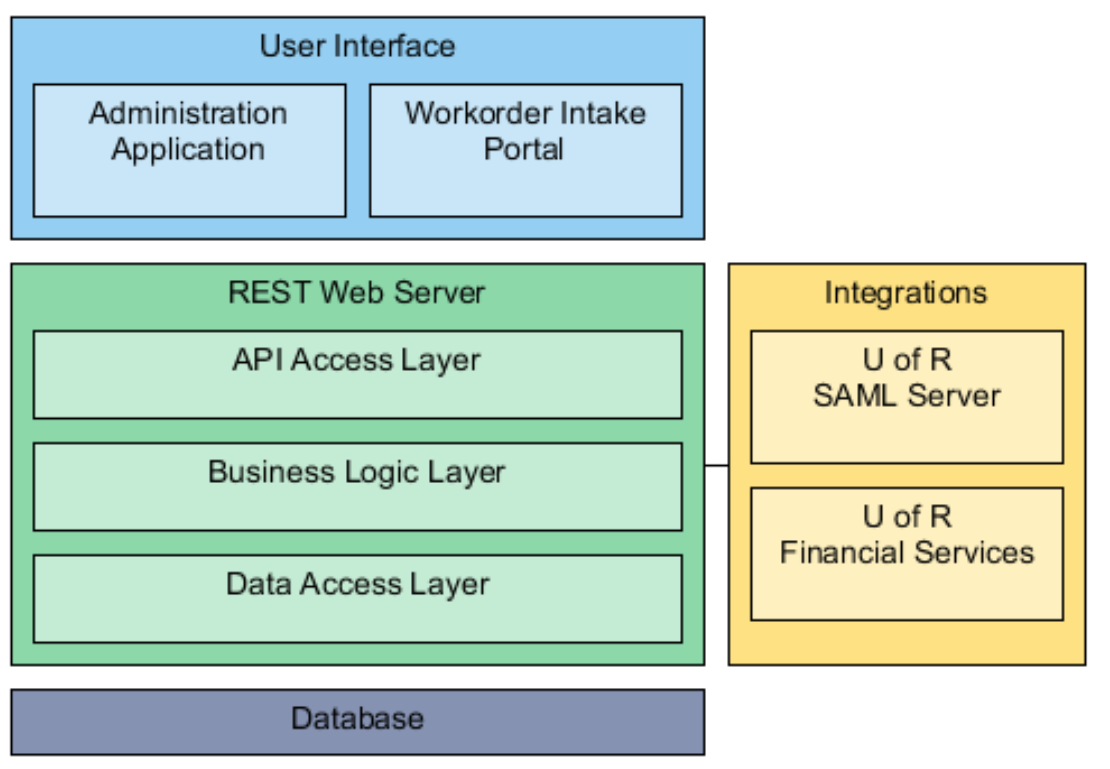
\includegraphics[width=3in]{front-back.png}\\
	\caption{Categories of the ERP Suite}
	\label{fig:tobias}
\end{figure}
\newline

On the front end, the client, who has the most control over the entire application. When the client log into the system upon start up, they have access to the main page displaying all necessary data for the particular day. In progress workorders, upcoming meetings and other related data can be quickly viewed. Clicking on a particular issue will navigate to a more in detailed view of the project. On the left side bar, the client can then access each particular section. 
\newline
{\setlength{\parindent}{0cm}

The first section is the Workorders page, where all workorders stored in the database can be accessed. Search and filtering options are available for the client when trying to locate specifics. Each workorder, displayed in a table with all necessary information, can be viewed, edited or deleted. When viewed in a closer look, tat particular workorder page is loaded, displaying all relevant information, including reference id, materials currently associated in the order, and all dates that apply. 
\newline
{\setlength{\parindent}{0cm}

The second section accessible by the left navigational bar is the time tracking feature, where the workshop manager can access the full calendar view of every time entry into the system, whether it is billable and non-billable hours. 

\subsection{Hardware Architecture}
Currently the application is a centralized system, with the client's operating machine and the server hosting the workshop's databases to be in the same location, thus allowing for the system to have a secure connection based on the university's internet. The type of server hosting the backend of the project is a REST web server, allowing the program to operate in a stateless environment, allowing the freedom of the application to transfer data to and from the database. This server is constructed using ASP.NET and entity framework, primarily written in the C\# language.   

\subsection{Software Architecture}
The three main pages are divided into their own sections, with each having their own specific connection to the back end, however, each page has a connection with each other as data is shared throughout the application. In total, each section requests and portrays the same data, but it is referenced in different ways. The following diagram showcases how each data table is related in the database.  
\begin{figure}[H]
	\centering
	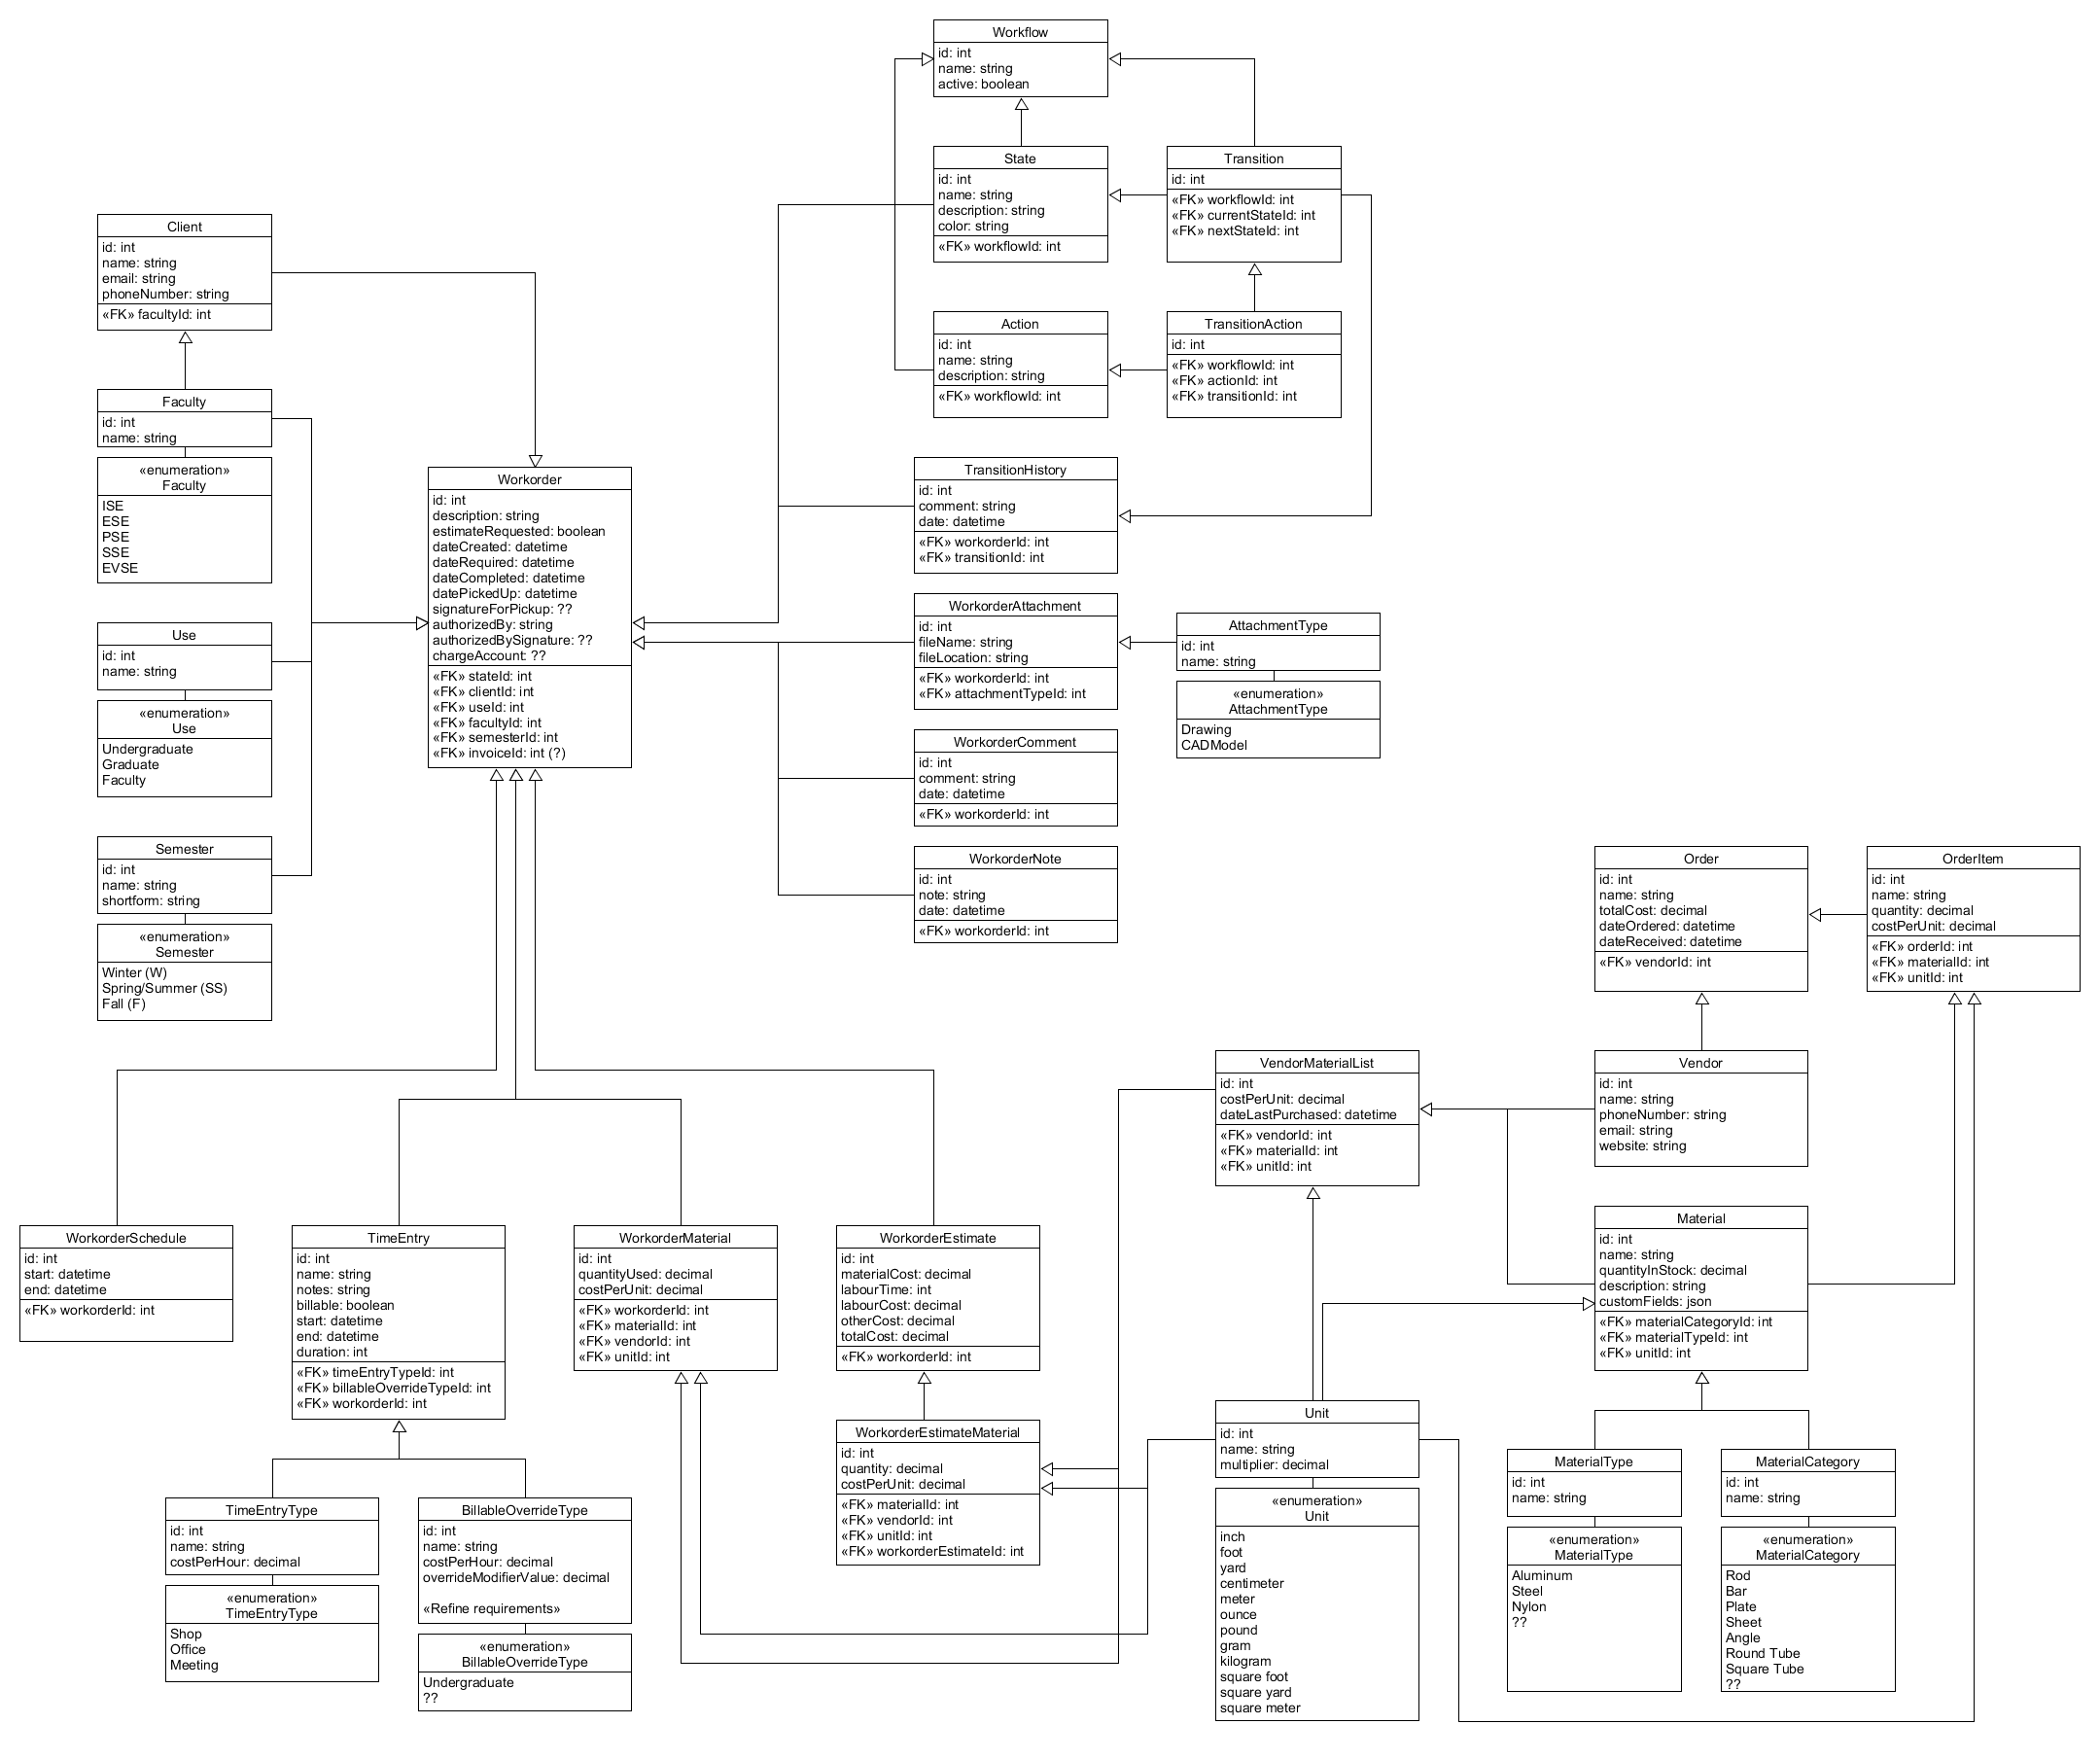
\includegraphics[width=7in]{class.png}\\
	\caption{Full class diagram of the ERP}
	\label{fig:tobias}
\end{figure}

Since each page accesses the database in different ways, data is requested for and received in different fashions. 
\subsubsection{Workorders}
On the workorders page, workorders are stored on the data are stored in the workorder table. Each entry includes the client, faculty, use, and semester information, as well as the dates of when the request was created and when the workorder is required to be finished, based on a workorder submission. The workorder table also stores the information associated to the workorder process, containing fields for statuses of a workorder, comments on the workorder, and any other additional attachments. The following figure showcases these relationships. 
\begin{figure}[H]
	\centering
	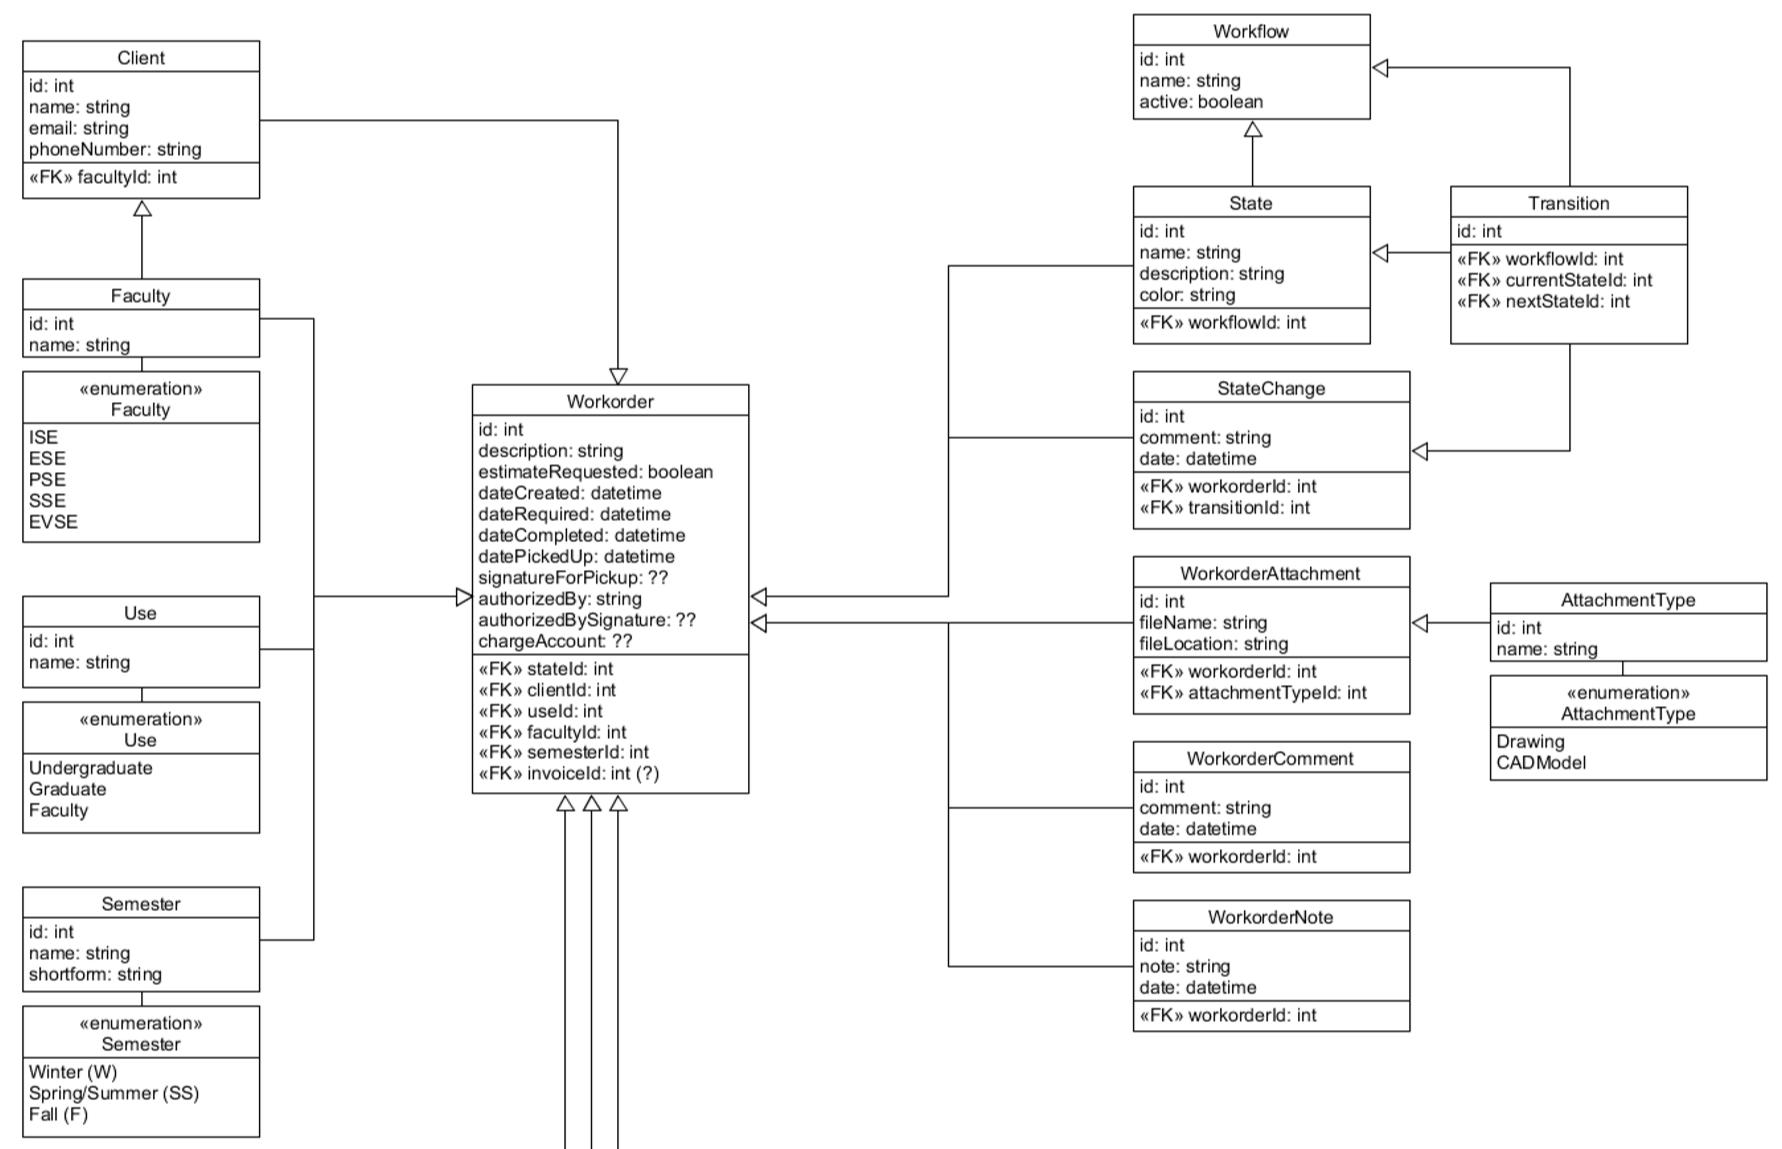
\includegraphics[width=5in]{workorder.png}\\
	\caption{Workorker Class Diagram}
	\label{fig:tobias}
\end{figure}

\subsubsection{Project Management}
For the project management system, each time entry involves having a specific type and the ability to insert billable time to an entry. Each Entry can then be considered an Event, which all those involved in the entry can be notified. The following class diagram showcases these relationships. 
\begin{figure}[H]
	\centering
	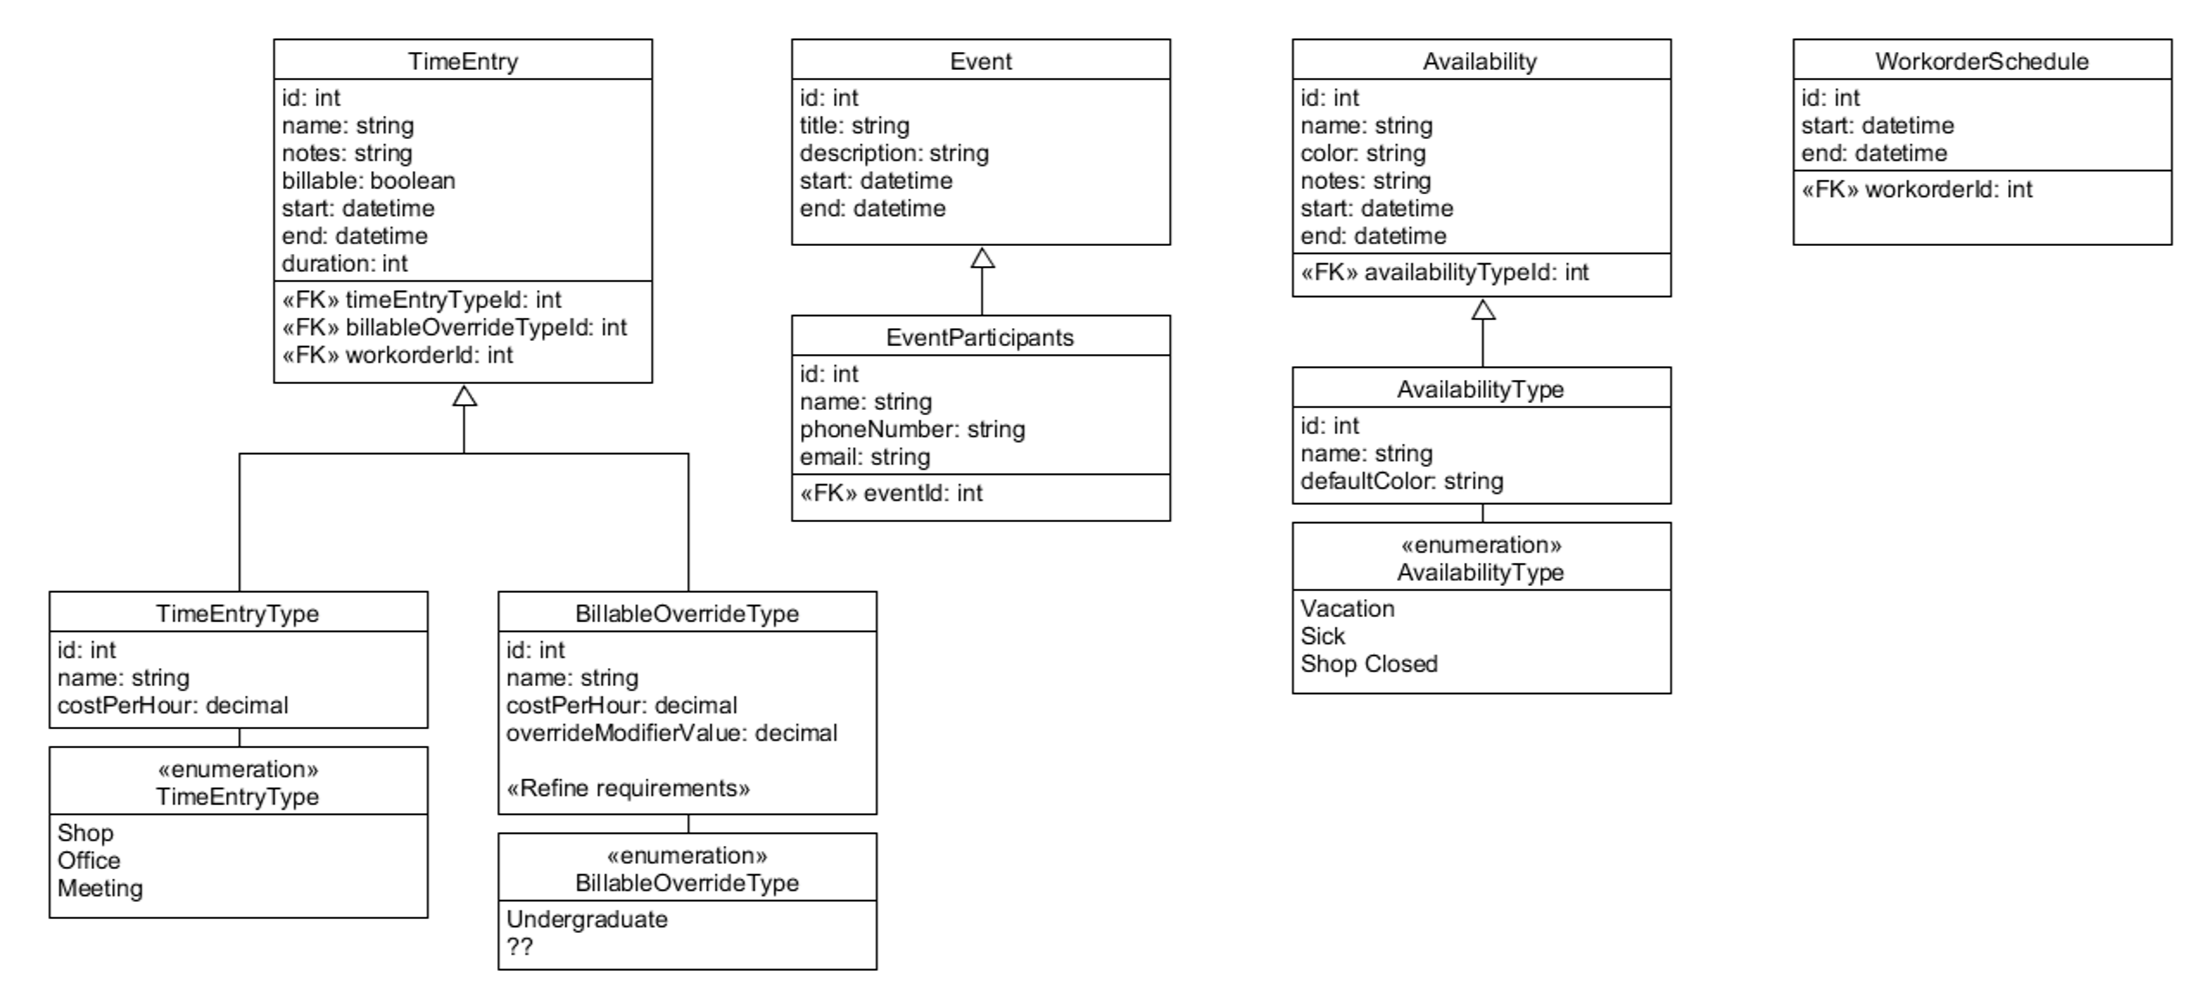
\includegraphics[width=5in]{project-management.png}\\
	\caption{Project Management Class Diagram}
	\label{fig:tobias}
\end{figure}

\subsubsection{Inventory}
The following class diagram showcases the inventory tables, and what goes into each particular material upon entry into the system. Every material has a type and falls into a particular category. There are a certain amount of it, stored using the appropriate unit. Each material is sold from a vendor, and each material is ordered from these specific vendors in specific orders. 
\begin{figure}[H]
	\centering
	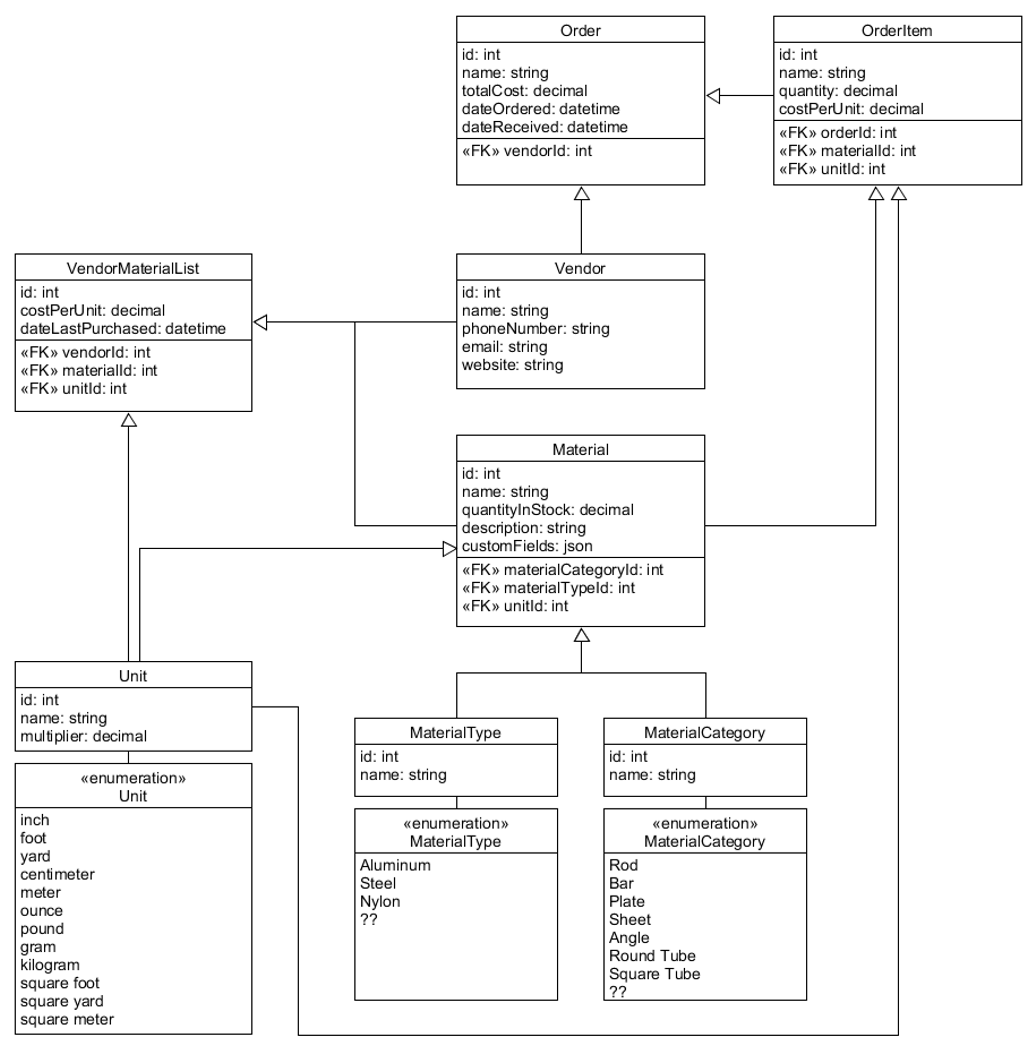
\includegraphics[width=5in]{Inventory.png}\\
	\caption{Inventory Class Diagram}
	\label{fig:tobias}
\end{figure}
\newpage

\section{System Design}
While creating the ERP suite, the following protocols and design patterns were used in order to perfect the web application such that is was effective in its functionality and comfortable to for the workshop manager to use. 

\subsection{Frontend Design}
The frontend of the program was created using a javascript framework called Vue.js, which is designed for web APIs and asynchronous CRUD functionality. While other similar frontend frameworks such as Razor Pages, which is the option provided by ASP.NET, and Angular, Google's own javascript framework, can provide the functionality that would be needed for the operation of the ERP suite, the decision to ultimately to use Vue was because of its extensive documentation and popularity in the web development world. It was the framework that had the most documented features available for use, allowing for more options and features be possible to implement inside the program. A typical Vue file has three distinct sections for the HTML code, styling and scripting, meaning that all of the features for a particular page is developed on a single page without having to switch in between files. This coupled with the fact that since Vue can run using a node packaging manager, it is able to be developed asynchronously in a development sever, are the reasonys as to why this framework was the primary choice for the ERP suite. As well, Vue allows for more personalization, without having to be locked into a template designed by a framework.

\subsubsection{UI Standards}
In the ERP suite, there are a set of user interface standards that are followed for consistency throughout the frontend design. 

\paragraph{Fonts}
Throughout the entire program, consistency in the font choice is crucial as to simplify the design of the program. The headings of the program as well as any standout text appearing on the site, such as in the side navigational bars on either side, use the Montserrat font. For the actual content of the program, the Roboto font was used. 

\paragraph{Palette}
In its current status, the ERP suite uses a blue-gray colour palette was used. While other, brighter colours are introduced throughout the application, these are primarily used for notification purposes, such as defining the status of workorders or reminders regarding deadlines approaching. To contrast these vibrant colours, a softer and calmer colour palette was needed such that notifications can still pop out for the user, signifying the importance of the task linked to them. The following figure showcases the particular palette used for the ERP suite. Attached are the hexadecimal numbers for each colour in the palette. 
\begin{figure}[H]
	\centering
	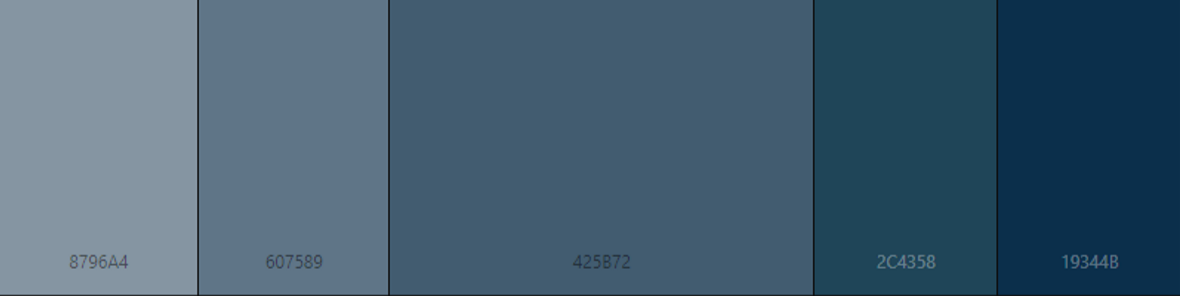
\includegraphics[width=5in]{palette.png}\\
	\caption{Colour palette used for the ERP suite}
	\label{fig:tobias}
\end{figure}

\subsection{Backend Design}
For the ERP suite, the backend aspect of the application is built using the ASP.NET web API framework. It uses the C\# programming language, and uses the ASP.NET packages and libraries allows for asynchronous access to the application's database as well as a connection to the frontend. Because of the nature of ASP.NET, the frontend can send requests during any time during runtime and can be a truly dynamic system.
\newline
{\setlength{\parindent}{0cm} 

Several other options were considered during the planning and design phases. other options for server side programming such as PHP, a completely server side language and Node.js, which is a javascript framework that allows for the use of the language as a server side scripting. However, both ultimately were not applicable for the purposes of this program. The main advantage of using ASP.NET over these options is is the use of the C\# language, and the access to the framework's libraries which are used throughout the program. 
\newline
{\setlength{\parindent}{0cm} 

The backend is broken up into 5 separate projects, which each providing a certain function which combine during runtime. The 5 different projects are API, Common, Models, Repositiories, and Services. 
\newline
{\setlength{\parindent}{0cm}
 
\subsubsection{API}
In the API project, the start up and controller code is located. The start up code is necessary for each web API to run, creating the access each library that will be used throughout the program. This program also configures the different database contexts, a feature of Entity Framework Core that enables the system to create a connection to the database in an abstract fashion. As well, connection with the frontend web pages are established. 
\newline
{\setlength{\parindent}{0cm} 

The way that ASP.NET is designed, controllers are used to create the endpoints which will send the necessary data to the frontend. Each endpoint is created using the CRUD methodology, using the GET, POST, PUT and DELETE requests. Each request states its type of message, and send a response back to the frontend, depending on the type of request made. Data that is requested by the frontend will be sent if the request is valid and if the particular entry exists. Before any requests are made by the user, they musted be authorized by the account controller. The system will return a 403 error if non-authorized requests are made. 

\subsubsection{Common}


\subsection{Database Design}
The main aspect for communicating with the system's database is Entity Framework Core. It allows the backend, which is written using ASP.NET, to work with and send requests to the database using .NET objects instead of the standard MySQL database language. This automates the database requests without having to write the SQL code for every request. Since the web API is designed in an asynchronous use, creating this layer of abstraction allows for the program run multiple requests with less actual scripting. 
\newline
{\setlength{\parindent}{0cm}

In its current design, the database will be hosted on the machine of the workshop manager located in the workshop, with the service connecting to the university internet when the application is running. Since the database does not need to store massive amounts of data, a larger server on university campus or a non-local server is not required but the application is open to these options in future implementations. 

\newpage
\section{External Interface Design}

\end{document}


